\chapter{Lezione 3 - Evoluzione dell'informatica giuridica.}

In questa lezione parliamo della storia di Internet, i nostri argomenti.

\begin{itemize}
    \item Cenni storici
    \item strumenti e attori
    \item l'identificazione sul web
\end{itemize}

\section{Cenni storici del web}

Partiamo dal primo argomento, cenni storici del web. La prima domanda è che cos'è Internet? \textbf {Internet è una rete internazionale formata dall'interconnessione di molte migliaia di reti di computer.}

Questa è la definizione che diamo di Internet. La cosa che sappiamo perfettamente ormai è che la rete ci permette di essere collegati e interconnessi in qualsiasi momento della giornata, in qualsiasi momento dell'anno. Ormai tutti, nessuno escluso, siamo connessi fra di noi attraverso una serie di dispositivi che fanno riferimento a Internet. 

Internet è stato l'ultimo dei mezzi di comunicazione di massa ad essere sviluppato e prima di proseguire vorrei farvi vedere un video. Si tratta di un video di Ted, Lessons Ted, che vi racconta di che cosa parliamo quando parliamo di Internet.

\subsection{Trascrizone video}
"Used by men, we're starting revolutions. We use it from our computers, our phones, even our cars. It's just there, all around us, all the time. But what is it exactly?

Well, first of all, the World Wide Web is not the Internet, even though the terms are often used interchangeably. The Internet is simply the way computers connect to each other in order to share information. When the Internet first emerged, computers actually made direct calls to each other. Today, networks are all around us, so computers can communicate seamlessly.

The communication enabled through the Internet has many uses, such as e-mail, file transfer, and conferencing, but the most common use is accessing the World Wide Web. Think of the Web as a bunch of skyscrapers, each representing a web server — a computer always connected to the Internet, specifically designed to store information and share it.

When someone starts a website, they are renting a room in this skyscraper, filling it with information and linking that information together in an organized way for others to access. The people who own these skyscrapers and rent space in them are called web hosts, but anyone can set up a web server with the right equipment and a bit of know-how.

There's another part to having a website, without which we would be lost in the city with no way of finding what we need. This is the website address, which consists of domain names — just like with a real-life address. Once you get where you want to go, the information stored in the websites is in web languages such as HTML and JavaScript.

When we find the website we're looking for, our web browser is able to take all the code on the site and turn it into words, graphics, and videos. We don't need to know any special computer languages because the web browser creates a graphic interface for us.

In a lot of ways, the World Wide Web is a big virtual city where we communicate with each other in web languages, with browsers acting as our translators. And just like no one owns a city, no one owns the Web — it belongs to all of us. Anyone can move in and set up shop. We might have to pay an Internet service provider to gain access, a hosting company to rent web space, or a registrar to reserve our web address. Like utility companies in a city, these companies provide crucial services — but in the end, not even they own the Web.

But what really makes the Web so special lies in its very name. Prior to the Web, we used to consume most information in a linear fashion. In a book or newspaper article, each sentence was read from beginning to end, page by page, in a straight line until you reached the end. But that isn't how our brains actually work. Each of our thoughts is linked to other thoughts, memories, and emotions in a loose, interconnected network — like a web.

Tim Berners-Lee, the father of the World Wide Web, understood that we needed a way to organize information that mirrored this natural arrangement, and the Web accomplishes this through hyperlinks. By linking several pages within a website — or even redirecting you to other websites to expand on information or ideas immediately as you encounter them — hyperlinks allow the Web to operate along the same lines as our thoughts.

The Web is so much a part of our lives because, in content and structure, it reflects both the wider society and our individual minds. And it connects those minds across all boundaries — not only ethnicity, gender, and age, but even time and space."


\subsection{Traduzione video}

Usato dagli uomini, stiamo iniziando rivoluzioni. Lo usiamo dai nostri computer, dai nostri telefoni, persino dalle nostre auto. È semplicemente lì, tutto intorno a noi, tutto il tempo. Ma che cos'è esattamente?

Innanzitutto, il World Wide Web non è Internet, anche se spesso i termini vengono usati come sinonimi. Internet è semplicemente il modo in cui i computer si connettono tra loro per condividere informazioni. Quando Internet è nato, i computer effettuavano vere e proprie chiamate dirette tra loro. Oggi, le reti ci circondano ovunque, quindi i computer possono comunicare in modo continuo e fluido.

La comunicazione resa possibile da Internet ha molti usi, come l’e-mail, il trasferimento di file e le videoconferenze, ma l’uso più comune è l’accesso al World Wide Web. Pensa al Web come a un insieme di grattacieli, ognuno dei quali rappresenta un \textit{web server}: un computer sempre connesso a Internet, progettato appositamente per archiviare e condividere informazioni.

Quando qualcuno crea un sito web, sta affittando una stanza in uno di questi grattacieli, riempiendola di informazioni e collegandole tra loro in modo organizzato, affinché altri possano accedervi. Le persone che possiedono questi grattacieli e affittano gli spazi sono chiamate \textit{web host} (provider di hosting), ma chiunque può creare un \textit{web server} con l’attrezzatura giusta e un po’ di competenze tecniche.

C'è un'altra parte essenziale per avere un sito web, senza la quale ci perderemmo nella città virtuale senza trovare ciò che ci serve: si tratta dell’indirizzo del sito web, che consiste in nomi di dominio — proprio come un indirizzo nella vita reale. Una volta arrivati dove vogliamo, le informazioni presenti nei siti web sono scritte in linguaggi come HTML e JavaScript.

Quando troviamo il sito che cerchiamo, il nostro browser web è in grado di interpretare tutto il codice presente sulla pagina e trasformarlo in testi, immagini e video. Non dobbiamo conoscere nessun linguaggio di programmazione, perché è il browser a creare per noi un'interfaccia grafica.

In molti modi, il World Wide Web è una grande città virtuale, dove comunichiamo usando linguaggi web, con i browser che fanno da traduttori. E proprio come nessuno possiede una città, nessuno possiede il Web: appartiene a tutti noi. Chiunque può ``trasferirsi'' e aprire il proprio ``negozio''. Potremmo dover pagare un provider di servizi Internet per accedere, un’azienda di hosting per affittare lo spazio web o un \textit{registrar} per prenotare il nostro indirizzo web. Come le aziende che forniscono elettricità o acqua in una città, queste aziende offrono servizi fondamentali — ma nemmeno loro possiedono il Web.

Ma ciò che rende davvero speciale il Web è già nel suo nome. Prima del Web, la maggior parte delle informazioni veniva consumata in modo lineare: in un libro o in un articolo di giornale, ogni frase veniva letta dall'inizio alla fine, pagina dopo pagina, in linea retta fino alla conclusione. Ma non è così che funzionano i nostri cervelli. Ogni nostro pensiero è collegato ad altri pensieri, ricordi ed emozioni, in una rete libera e interconnessa — proprio come una ragnatela.

Tim Berners-Lee, il padre del World Wide Web, capì che avevamo bisogno di un modo per organizzare le informazioni che rispecchiasse questa disposizione naturale. Il Web realizza questo grazie ai collegamenti ipertestuali (\textit{hyperlink}). Collegando varie pagine all’interno di un sito — o indirizzandoti verso altri siti per approfondire subito concetti e idee — i collegamenti ipertestuali permettono al Web di funzionare secondo la stessa logica del pensiero umano.

Il Web fa così tanto parte delle nostre vite perché, sia nei contenuti che nella struttura, riflette sia la società in generale che le nostre menti individuali. E collega queste menti oltre ogni confine — non solo etnico, di genere o di età, ma anche di tempo e spazio.

\subsection{Continuazione Lezione}

Come avete visto,internet e il World Wide Web non sono esattamente la stessa cosa. Internet, come lo conosciamo oggi, si diffonderà nel 1992, ma già da molto tempo erano iniziate una serie di attività che hanno portato a quello che Internet è oggi. 

Facciamo quindi un passo indietro e torniamo alle origini.

\subsection{Le origini di Internet}

Le origini sono Arpanet. 
Nel 1958, la DARPA( Defense Advanced Research Project Agency) sviluppa un sistema di collegamento voluto fortemente dagli Stati Uniti che aveva come obiettivo quello di tenere sotto controllo, attraverso una rete, le basi militari. 

Nel 1969 si iniziano a collegare i primi nodi delle università importanti, l'Università della California, Stanford Research Institute, Santa Barbara, Utah. 

Che cosa ha di particolare Arpanet e qual è la sua differenza rispetto al moderno Internet? Arpanet è caratterizzato da nodi autonomi operativi in situazioni di instabilità. Come ho detto, Arpanet non è ancora la nostra rete ed è, come ho detto, inizialmente nasce per delle esigenze di carattere militare degli Stati Uniti ed è a partire dagli anni 70 che inizia ad essere invece utilizzata anche al di fuori di quello che è l'ambito militare, proprio dalle università. 

Le origini di Internet. \par
\begin{itemize}
    \item Nel 1970 si iniziano a trasmettere i primi messaggi di posta, i dati e i programmi.
    \item Nel 1980 viene creata la Rete delle Reti, 213 computer collegati fra di loro.
    \item Nel 1981 da ARPANET ad Internet
    \item Nel 1983 l'ARPANET dona Internet alle università americane e in questo modo dà il primo punto di svolta a questa nuova realtà della comunicazione.
\end{itemize}

Ricordiamoci sempre che Internet è un mezzo di comunicazione di massa e lo è realmente diventato. Il passo successivo è il coinvolgimento dell'Europa. Fino adesso Internet, la Rete, è stata una prerogativa degli Stati Uniti. A partire dagli primi anni 80 si coinvolge anche l'Europa attraverso il CERN (Centro Europeo delle Ricerche) e il CERN collabora attivamente allo sviluppo della Rete.
\
subsubsection{Le origini di NFSnet e web}.

\begin{itemize}
    \item Nel 1985 NFS (National Science Foundation) collega le università.
    \item Nel 1990 la Rete della National Science Foundation sostituisce Arpanet.
    \item Nel 1991 il CERN, (Consiglio Europeo per la Ricerca Nucleare) progetta la Rete, ed è quindi nel 1991 che si avvia realmente Internet per tutti.
    \item Nel 1993 Internet è per tutti
\end{itemize}

Come è nata la  ricerca del CERN?

Nel 1989 il fisico informatico britannico Tim Barners-Lee propone al CERN di Ginevra il suo progetto per un'iniziativa di condivisione ipermediale dell'informazione globale via Internet. La prima pagina web viene messa a disposizione proprio nel 1991. 

Nel 1993 Internet è finalmente per tutti. 

Adesso voglio mostrarvi una timeline storica (fig. \ref{fig: Internet Timeline}) per darvi l'idea di quello che è stato il passaggio dalle origini fino ai nostri giorni di Internet. 

\begin{figure}[ht]
    \centering
    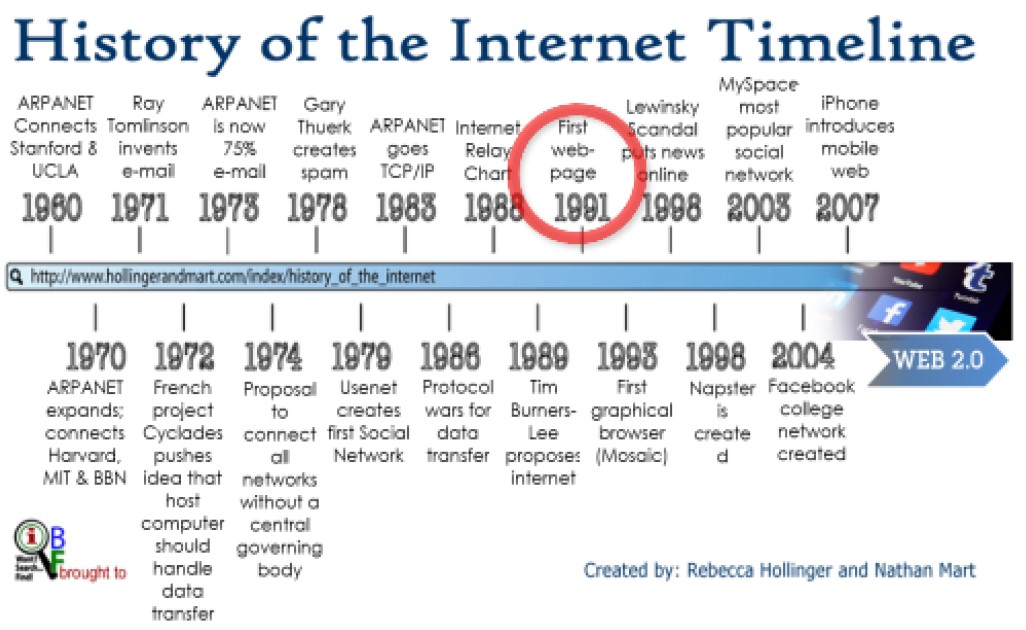
\includegraphics[width=0.9\linewidth]{images/03_lez_fig_01.jpg}
    \caption{History of Internet Timeline}
    \label{fig: Internet Timeline}
\end{figure}

Partiamo dal 1960 e arriviamo al 2007 con il web 2.0. 
Una delle date da ricordare più importanti è il 1991, data nella quale è stata pubblicata la prima web page.

Il nostro spunto di riflessione per questa prima parte della lezione è; quando è nato il moderno Internet? 

\subsection{Chi sono i principali strumenti e i principali attori di Internet?}

In questa seconda parte parleremo proprio di questi strumenti e attori. \par

\begin{itemize}
    \item Il World Wide Web
    \item gli Internet Service Provider
    \item i browser
    \item i motori di ricerca
    \item gli utenti
\end{itemize}

Come avete visto ho indicato gli utenti tra gli strumenti e gli attori del web perché nel web 2.0 gli utenti hanno un ruolo fondamentale di condivisione. Oggi gli utenti non sono più soltanto fruitori di ciò che accade su Internet, ma sono essi stessi artefici di quello che viene pubblicato. E partiamo quindi a cercare di definire chi sono tutti questi soggetti.

\subsubsection{World Wide Web}

Il  World Wide Web è il servizio di Internet che permette di navigare e usufruire di contenuti multimediali collegati tra loro (link) e di altri servizi. Il World Wide Web è il sistema che permette la condivisione di documenti ipertestuali e multimediali. 
Che cosa significa documenti ipertestuali e multimediali? 
Vuol dire che non si tratta soltanto di testo scritto ma che all'interno di questi documenti sono compresi anche altre immagini, suoni, altre forme di comunicazione e che tutte quante arrivano a costituire un unico documento, continuiamo a chiamarlo così utilizzando un termine tradizionale, ma fruibile in più modi da parte dell'utente.

Per accedere al World Wide Web si utilizza un software particolare detto browser. Quindi il web è un insieme di server web interconnessi.

\subsubsection{Web server}

I web server sono delle applicazioni software in esecuzione su un server che possono gestire le richieste di trasferimento di pagine web a un client. 

Ma i documenti dove sono? 

I documenti sono genericamente detti pagine web e sono memorizzati in porzioni della memoria dei server e sono raggruppati in insiemi più o meno uniformi per aspetto o per contenuti che sono organizzati secondo una qualche struttura. Questi sono detti siti. 
Per essere accessibili le pagine web vengono costruite con dei linguaggi descrittori particolari che permettono di specificare sia il contenuto della pagina, sia il loro formato di visualizzazione sul browser dell'utente.

Da questo punto di vista la visualizzazione è diversa quando l'utente è davanti allo schermo di un computer oppure quando è davanti ad un dispositivo mobile.

Vi sarete resi perfettamente conto ormai che le applicazioni su dispositivo mobile sono sempre più diffuse, che il modo di accedere, il modo di visualizzare i siti è completamente diverso.

La comunicazione tra utente e server così come il trasferimento tra le pagine web sono regolate da dei protocolli di trasferimento così detti e le singole risorse che sono disponibili sulla rete sono individuate univocamente da una serie di caratteri di identificazione universale.

In particolare la URL, \textbf{Uniform Resource Locator}, consente di specificare il nome e la posizione del documento. Poi torneremo su questo punto per comprendere come sia possibile l'identificazione univoca. La caratteristica principale della rete web è che i nodi che la compongono sono tra loro collegati tramite i link, i cosiddetti collegamenti ipertestuali, e in questa maniera formano un enorme ipertesto in modo tale che gli utenti possano navigare e usufruire di contenuti amatoriali e professionali multimediali e non.

La facile reperibilità delle informazioni è resa possibile dalla diffusione, facilità d'uso ed efficienza dei motori di ricerca e dei web browser appunto, in un modello di architettura di rete definito client-server. E quindi torniamo al nostro web server. Un server web, come detto prima, è un'applicazione software che permette di gestire le richieste di trasferimento di informazioni di pagine web di un client. Vediamo in fig. \ref{fig:Tipologie di server web} quali sono i web server più diffusi oggi nel mondo.

\begin{figure}[ht]
    \centering
    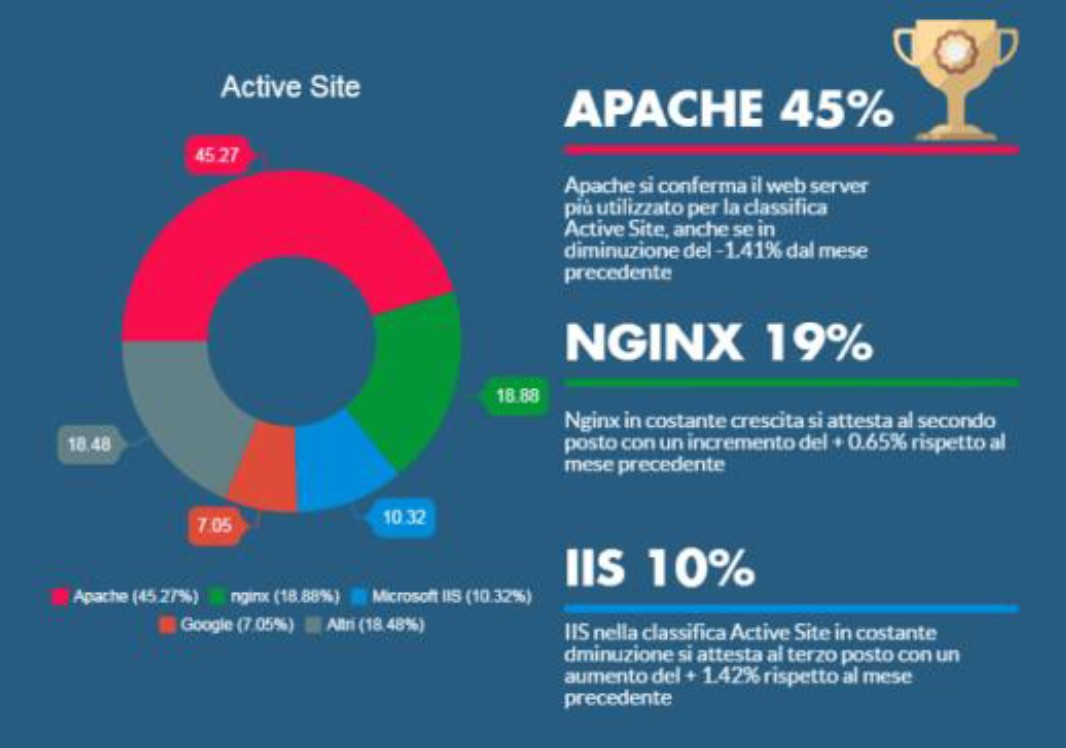
\includegraphics[width=0.8\linewidth]{images/03_lez_fig_02.jpg}
    \caption{Titologie di server web}
    \label{fig:Tipologie di server web}
\end{figure}

I web server più utilizzati nel dicembre 2016 erano principalmente Apache con una diffusione del 45\% seguiti da NGINX al 19\% e poi gli altri, IIS il 18\% e così via. 

Ecco qui un altro schema di riferimento in cui c'è il numero di presenze (fig. \ref{fig:presenza di server web}).
\begin{figure}[ht]
    \centering
    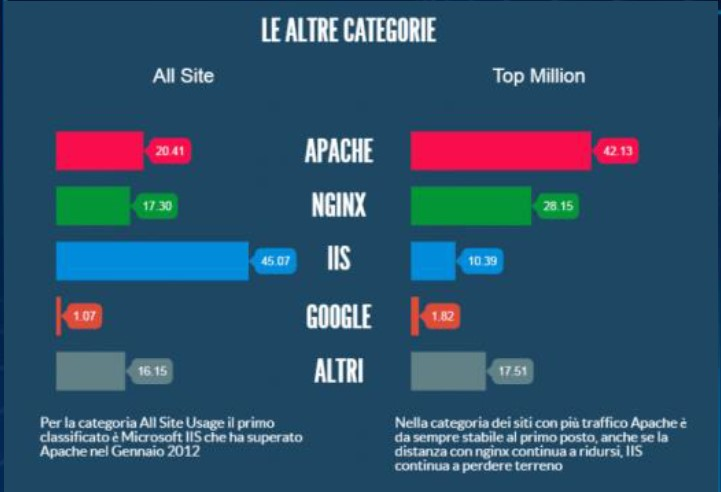
\includegraphics[width=0.8\linewidth]{images/03_lez_fig_03.jpg}
    \caption{Presenza di server web}
    \label{fig:presenza di server web}
\end{figure}

Continuamente nascono dei nuovi server, non sempre riescono ad avere una diffusione tale da aggredire quella che è attualmente la distribuzione.

\subsubsection{ISP Internet Service Provider}

Oltre ai server ci sono gli internet service provider, società che a pagamento permettono l'accesso a internet e forniscono altri servizi come email, spazi per la creazione di siti e così via. Un internet service provider è un fornitore di servizi internet appunto e cioè una struttura a carattere commerciale o un'organizzazione che offre agli utenti, persone fisiche e imprese, l'accesso a internet a pagamento con la stipula di contratti di fornitura. Di solito per la connessione a un internet service provider si utilizza una connessione remota attraverso una linea telefonica, banda larga o attraverso tutte quelle che sono le forme di connessione che la tecnologia riesce a mettere a disposizione degli utenti.

Gli internet service provider permettono o offrono anche dei servizi aggiuntivi fondamentali per la gestione e la fruibilità, cioè la posta elettronica, spazi per la creazione di siti web e quant'altro.

Gli internet service provider non sono tutti uguali fra loro, quelli di primo livello costituiscono la dorsale principale di internet e a questi sono connessi gli internet service provider di secondo livello che fungono da punti di connessione.

Dal 2000 in poi il mercato dell'accesso a internet ha avuto una crescita esponenziale e gli internet service provider hanno aggiunto servizi su servizi e non sono più solo dei punti di accesso, cosa che rimane comunque fondamentale, ma  danno tutta una serie di altre possibilità e in questo modo a seconda delle possibilità che offrono si fanno anche concorrenza fra di loro.

Ogni paese ha i suoi, in Italia l'associazione italiana internet provider, in UK la ISPA UK, in Francia AFPI e in Europa in generale l'euro ISPA. (fig. \ref{fig:Associazioni_ISP}) \par

\begin{figure}
    \centering
    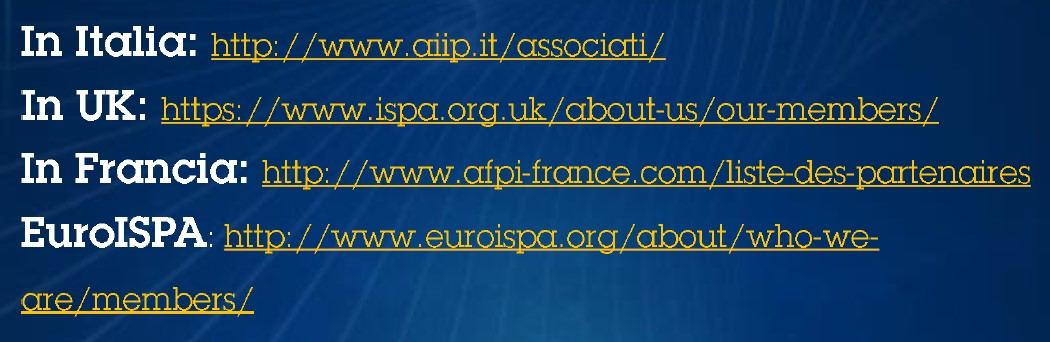
\includegraphics[width=1\linewidth]{images/03_lez_fig_04.jpg}
    \caption{Associazioni ISP}
    \label{fig:Associazioni_ISP}
\end{figure}


\subsubsection{Browser}
I browser sono applicazioni per il recupero, la presentazione, la navigazione di risorse sul web. 
Esempi sono  Google, Firefox, Safari, Microsoft Edge, Opera.

Il browser è fondamentale per poter accedere alla risorse messa a disposizione sul web. Da un lato il programma implementa le funzionalità del client e dall'altro consente la visualizzazione dei risultati, dei contenuti ipertestuali che vengono ricercati.

\subsubsection{Motori di ricerca}
Il motore di ricerca è un sistema automatico che su richiesta analizza un insieme di dati raccolti e restituisce un indice dei contenuti disponibili. I motori di ricerca più utilizzati nel 2017 sono:

\begin{itemize}
    \item Google
    \item Bing
    \item Qwant
    \item Yandex
    \item Ecosia
    \item Duck Duck GO
\end{itemize}

Sono motori di ricerca che hanno delle grandi similitudini fra loro ma anche delle differenze e sono le differenze sulle quali si basa la concorrenza. 

Come ho detto prima, Google assolutamente ha sbaragliato tutti, se consideriamo, il numero di accessi che ha quotidianamente è assolutamente di molto al di sopra di tutti gli altri.

Le caratteristiche di diversificazione sono la velocità, oppure la quantità di notizie di risultati che vengono restituiti, le modalità innovative di presentazione dei risultati stessi.

Avrete forse in passato sentito parlare di una vicenda che ha riguardato le modalità di presentazione dei risultati da parte di Google. Se navigate provate a googlare (è un termine ormai entrato nell'uso comune, non soltanto in Italia ma anche in altri paesi) e provate a cercare Google Spain troverete una serie di risultati relativamente ad una sentenza molto importante della Corte di Giustizia dell'Unione Europea che ha affrontato il tema del trattamento dati personali.

Torneremo su questo argomento in un'altra lezione relativamente al trattamento dati personali da parte dei motori di ricerca e la loro presentazione senza limitazioni di tempo anche a distanza di molti anni. Sulla base di questo si è elaborato un concetto di diritto all'oblio, diritto a essere dimenticati da web, che ha delle caratteristiche diverse rispetto a ciò che è mai stato in precedenza.

Torniamo ai motori di ricerca, i quali:

\begin{itemize}
    \item permettono l'organizzazione dei contenuti e il loro collegamento
    \item stabiliscono una relazione tra la ricerca dell'utente e le informazioni
    \item restituiscono una lista di riferimenti con una breve descrizione di quello che è il contenuto
    \item Attraverso degli hyperlink aprono altri siti o risorse
    \item Per ricordare quali sono state le precedenti ricerche dell'utente installano dei cookies, delle piccole stringhe di testo, che consentono di ricordare quali sono state le ultime ricerche dell'utente e permettono così di velocizzare le attività di ricerca.
\end{itemize}


\begin{figure}[ht]
    \centering
    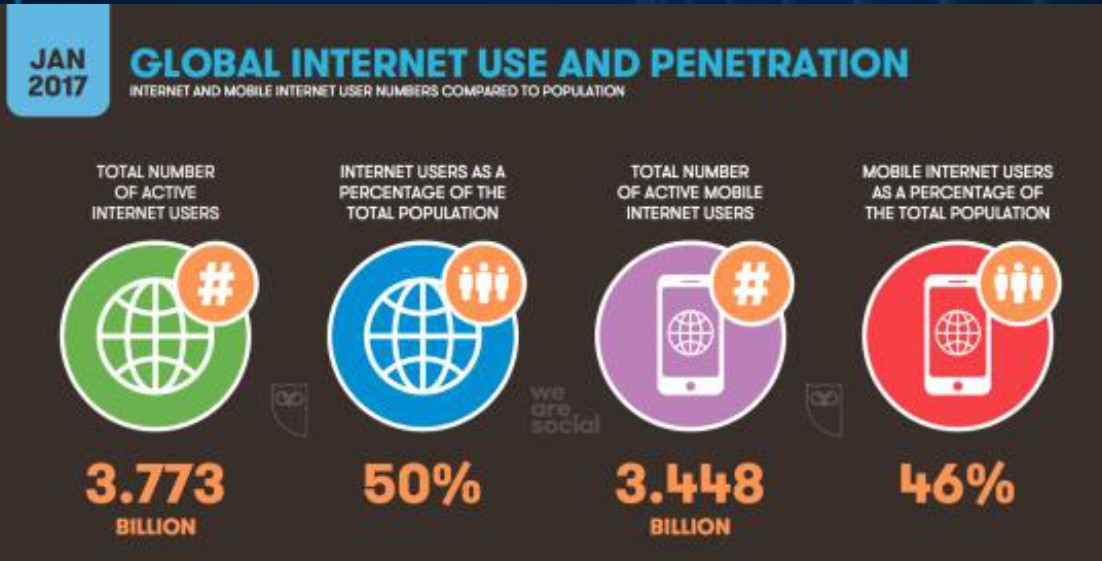
\includegraphics[width=1\linewidth]{images/03_lez_fig_05.jpg}
    \caption{Penetrazione globale di internet}
    \label{fig:penetrazione_globale_internet}
\end{figure}

Nel gennaio 2017 l'uso e la penetrazione globale di internet è descritta in questa slide (fig. \ref{fig:penetrazione_globale_internet}). 

Su 3 miliardi 773 milioni di utenti attivi su internet, il 50\% è la percentuale sulla popolazione globale, il totale dei dispositivi mobili attivi è 3 miliardi e 448 milioni e i dispositivi mobili sono una percentuale del 46\%. 

In quest'altra slide potete vedere la diffusione di internet in base alle regioni del mondo (fig. \ref{fig:diffusione_internet}):
\begin{figure}[ht]
    \centering
    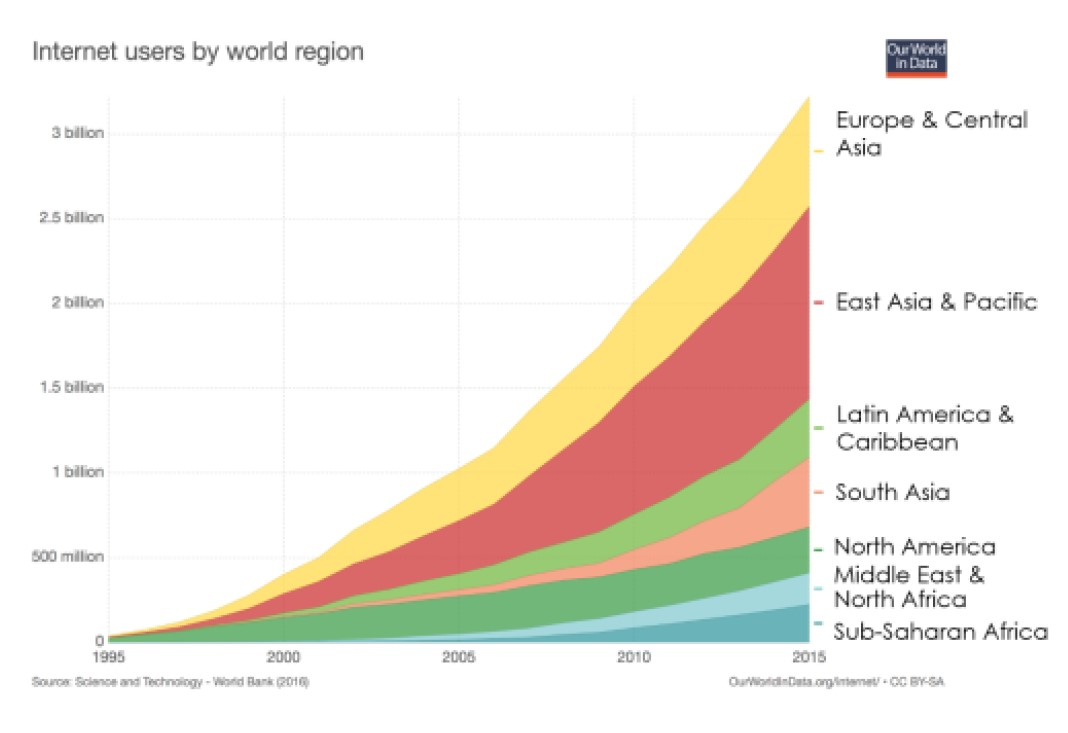
\includegraphics[width=0.9\linewidth]{images/03_lez_fig_06.jpg}
    \caption{Diffuzione di internet negli anni}
    \label{fig:diffusione_internet}
\end{figure}


Europa e Asia centrale, 3 miliardi, Est Asia e Pacifico 2 miliardi circa, America Latina e Caraibi 1 miliardo, Asia del sud, Nord America e così via. Questa è la penetrazione e soprattutto il cambiamento, la curva ascendente che c'è stata tra il 1995 e il 2015. I numeri sono cresciuti in maniera veramente eccezionale. 

Il nostro spunto di riflessione per questa seconda parte della lezione è chi fornisce l'accesso a internet ai cittadini?

\subsection{Identificazione sul web}

Abbiamo accennato all'inizio della nostra lezione che è fondamentale sul web l'accessibilità effettiva alle risorse che ci sono ed è quindi necessario avere una identificazione univoca di ogni utente, di ogni sito e  per questo bisogna rispettare delle regole.

\subsubsection{Gli indirizzi in internet.}

Per accedere ad una risorsa su internet è necessario conoscerne la localizzazione, cosiddetto indirizzo IP.

La URL (Uniform Resource Locator) identifica l'indirizzo sulla rete in modo univoco.

Vedete su questa slide una descrizione di che cos'è la URL (fig. \ref{fig:descrizione_URL}).

\begin{figure}[ht]
    \centering
    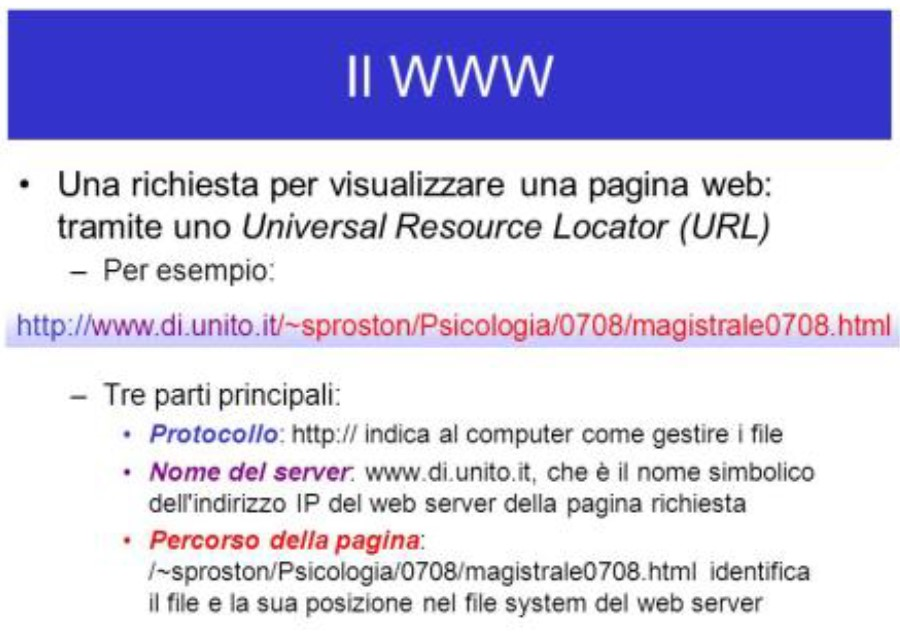
\includegraphics[width=0.9\linewidth]{images/03_lez_fig_07.jpg}
    \caption{Descrizione URL}
    \label{fig:descrizione_URL}
\end{figure}

Ad esempio, http://www.di.unito.it è un indirizzo che è composto di tre parti principali.

Il protocollo http indica al computer come gestire i file, il nome del server www.di.unito.it è il nome simbolico dell'indirizzo IP del web server della pagina richiesta e poi c'è il percorso della pagina.

Tutta questa serie di caratteri alfanumerici identificano il file e la sua posizione nel file system del web server. 
Gli indirizzi in internet sono sempre gli stessi in un certo senso ma un cambiamento importante nel corso del tempo è stata la individuazione dei DNS (domain name server). 
Il DNS consente l'individuazione univoca con un linguaggio alfanumerico comprensibile con un passaggio da codice numerico a una stringa di testo. Grazie ai domain name server per raggiungere i siti si possono utilizzare i nomi a dominio invece degli indirizzi IP, cioè in altri termini ogni sito è raggiungibile attraverso un IP numerico ma ciò che l'utente digita è un nome e questo nome viene riconosciuto come collegato in maniera univoca a quel determinato indirizzo e quindi consente di accedere alla risorsa.

Anche i nomi a dominio così come gli indirizzi IP devono essere univoci, per garantirlo la loro assegnazione è affidata a diversi organismi centrali.

Ma quali nomi a dominio esistono e cosa significano le varie estensioni dei nomi a dominio? I nomi a dominio hanno una struttura gerarchica che adesso vediamo.

\subsubsection{La struttura dei DNS}

\begin{itemize}
    \item Ci sono prima di tutto i top level domain (TLD) o domini di primo livello
          \begin{itemize}
              \item generici gTLD come .org, .net e com. Questi top level domain sono assegnati da una struttura internazionale chiamata ICANN
              \item country code top level domain ccTLD che sono i domini caratteristici dei vari paesi, quindi abbiamo .it, .at, .fr, .uk. Ogni paese ha un dominio caratteristico.
          \end{itemize}
    \item Dopodiché abbiamo i second level domain, i domini di secondo livello
    \item e poi il third level domain (sub domain) che sono definiti nella rete locale.
\end{itemize}

Sia i general gTLD, sia i country code ccTLD sono domini di primo livello. \par

I general Top level domain (gTLD) riguardano:
\begin{itemize}
    \item .com organizzazioni commerciali,
    \item .edu riguardano gli enti di ricerca alle università,
    \item .gov enti governativi,
    \item .int organizzazioni internazionali,
    \item .mil enti militari,
    \item .net enti di gestione della rete,
    \item .org enti diversi di volontariato, associazioni senza scopo di lucro e quant'altro
    \item i domini nazionali, .it, .fr, .uk, .de, ...
    \item .eu le istituzioni europee hanno un dominio EU che è caratteristico
\end{itemize}

\subsubsection{L'assegnazione dei general top level domain (gTLD)}

L'assegnazione dei general top level domain e quindi l'assegnazione degli indirizzi di rete curata dall'\textbf{ICANN, Internet Corporation for Assign Names and Number}, il sito dove andare a verificare, a studiare, esaminare di che cosa si tratta è www.ican.org. 

Parleremo meglio di ICANN in una prossima lezione, ma in questa lezione ci sono alcune indicazioni fondamentali che è bene che voi abbiate.
%-------------------------------------------------------
L'ICANN è stato istituito nel 1998 e incaricato dalle autorità governative degli Stati Uniti. Al giorno d'oggi è invece un ente di gestione internazionale. Potete notare, se fate mente locale a quanto abbiamo detto precedentemente in questa lezione, che l'origine di tutto ciò che riguarda il nostro internet è partita dagli Stati Uniti.

Il coinvolgimento degli altri paesi, in particolare dell'Unione Europea, è avvenuto in un secondo momento e a questo ha corrisposto una effettiva globalizzazione del mondo internet. Ma è per questa ragione che anche gli enti che si occupano della gestione di internet in prima battuta sono nati negli Stati Uniti e in prima battuta sono nati su indicazione degli organismi pubblici statunitensi. Abbiamo parlato dell'Arpanet che partiva dalle autorità militari, ma anche il soggetto che assegna i nomi di dominio, ICANN, è stato in prima battuta incaricato dal governo degli Stati Uniti. Il fatto che oggi sia un ente di gestione internazionale è sicuramente una garanzia di maggiore coinvolgimento anche degli altri Stati.

ICANN (Internet Corporation for Assigned Names and Numbers) ha l'incarico di assegnare gli indirizzi IP ed identificare e gestire i gTLD.

\subsubsection{assegnazione dei ccTLD}

L'assegnazione dei ccTLD, cioè i Country Code Top Level Domain, è invece curata dai Registrar locali. In Italia la Naming Authority fa capo al CNR (Consiglio Nazionale delle Ricerche), e opera con il Ministero delle Poste e delle Telecomunicazioni (www.nic.it).

L'assegnazione dei Country Code Top Level Domain è in ogni Stato assegnata ad un registrar locale. In ogni Paese quindi c'è un registro locale e in Europa per l'assegnazione dei domini EU c'è l'EURID che è il registrar dei country code top level domain .eu (eurid.eu/en/).

Interessante è il CENTR, l'associazione dei registri dei ccTLD europei che raccoglie tutti quanti i registrar locali. (www.centr.org).

I registrar hanno un contratto/accordo con ICANN, tutti quanti ad eccezione della Germania e della Gran Bretagna. Quindi se andate a fare una verifica sui vari siti dei registrar locali, vedrete che fanno riferimento all'ICANN per mantenere un coordinamento e anche per valutare e verificare quali sono le regole da applicare. La Gran Bretagna e la Germania invece sono completamente autonomi.

\subsubsection{Registrar WHOIS}
I registrar svolgono una funzione molto importante, la funzione WHOIS. 

I registrar mantengono il database in cui sono indicati i dati dei titolari e dei nomi a dominio. Il mantenimento di un database è molto importante, non si tratta soltanto di tenere l'indicazione dei vari indirizzi assegnati, dei nomi di dominio assegnati, ma si tratta di conservare le informazioni relative ai titolari di questi siti e di questi domini. E' possibile un'interrogazione di questi database da parte di chi ha interesse a sapere chi sia il titolare di un nome a dominio, ma i nomi a dominio possono attivare la cosiddetta funzione privacy. 

La funzione privacy è una funzione in base alla quale a fronte di una interrogazione del motore di ricerca si possono avere alcune informazioni legate al titolare della registrazione, ma non tutte. È una funzione che mantiene riservato il nominativo, la denominazione del titolare. Questo ovviamente garantisce il titolare del nome di dominio, ma può mettersi in conflitto con quelle che può essere l' esigenza degli utenti di conoscere chi c'è dietro a un determinato dominio. La questione può interessare quando c'è un trattamento di dati personali, di dati di altri, quando attraverso un determinato sito vengono commessi degli illeciti, quando vengono diffuse delle fake news. L'oscuramento delle informazioni relative al titolare può impedire l'esercizio di altri diritti. 

Ne riparleremo in una prossima lezione, ma intanto il nostro spunto di riflessione per questa terza parte della lezione.

Chi è il responsabile dell'assegnazione di nomi a dominio CCTLD? 

Ora andiamo al riepilogo degli spunti di riflessione.

\begin{itemize}
    \item Quando è nato il moderno Internet?
    \item Chi fornisce l'accesso a Internet ai cittadini?
    \item Chi è il responsabile dell'assegnazione di nomi a dominio ccTLD?

\end{itemize}
La nostra lezione termina qui.